\documentclass[11pt]{article}

\usepackage[margin=2cm]{geometry}

\usepackage{graphicx}

\usepackage{booktabs}

\usepackage{hyperref}

\usepackage[T1]{fontenc}

\usepackage[utf8]{inputenc}

\title{Auditoría de universos de Santa Ana Xalmimilulco}

\author{Proyecto Atoyac - salida reproducible}

\date{\today}

\begin{document}

\maketitle

\section{Objetivo y jerarquía}

El universo original de Santa Ana es el canónico. MH es una capa ya filtrada de referencia. El filtro explícito nuevo es una alternativa analítica trazable. Ningún conjunto constituye evidencia de descarga o contaminación.

\section{Pipeline único}

La ejecución completa se realiza con \texttt{python scripts\textbackslash run\_santa\_ana\_pipeline.py}. Primero SAIC define las familias manufactureras textiles; después esas familias y los servicios 8122 se buscan en DENUE; finalmente se aplican las exclusiones y señales estrictas aprendidas.

\section{Tamaños}

Los vocabularios, codigos SCIAN y prioridades se leen desde \texttt{config\textbackslash filtros\_textiles\_santa\_ana}. Ningun script historico es entrada de esta ejecucion.

\begin{tabular}{ll}
\toprule
conjunto & registros \\
\midrule
denue\_2026\_santa\_ana\_total & 1732 \\
denue\_textil\_candidatos & 361 \\
universo\_canonico\_original\_santa\_ana & 38 \\
mh\_filtrado & 49 \\
mh\_filtrado\_con\_id & 43 \\
mh\_filtrado\_sin\_id & 6 \\
universo\_relevante\_filtro\_explicito & 293 \\
registros\_revisar\_filtro\_explicito & 18 \\
union\_comparacion & 322 \\
\bottomrule
\end{tabular}

\section{Resultado del filtro explícito}

\begin{tabular}{lll}
\toprule
categoria\_filtro & relevancia\_ambiental & registros \\
\midrule
excluir\_comercio & excluir & 795 \\
fuera\_filtro & fuera & 589 \\
maquila\_textil & media & 171 \\
produccion\_textil & media & 114 \\
excluir\_actividad\_no\_objetivo & excluir & 29 \\
revisar\_lavado\_generico & revisar & 16 \\
excluir\_lavado\_no\_textil & excluir & 8 \\
lavado\_acabado\_textil & alta & 8 \\
revisar\_maquila\_sola & revisar & 2 \\
\bottomrule
\end{tabular}

\section{Canónico original frente a MH filtrado}

\begin{tabular}{ll}
\toprule
comparacion\_canonico\_vs\_mh & registros \\
\midrule
canonico\_y\_mh & 7 \\
mh\_sin\_id & 6 \\
solo\_canonico\_original & 31 \\
solo\_mh\_filtrado & 36 \\
\bottomrule
\end{tabular}

\section{Canónico original frente al filtro explícito}

\begin{tabular}{ll}
\toprule
comparacion\_canonico\_vs\_foco & registros \\
\midrule
canonico\_y\_foco\_estricto & 18 \\
solo\_canonico\_original & 20 \\
solo\_foco\_estricto & 275 \\
\bottomrule
\end{tabular}

\section{Reglas de la alternativa analítica}

\begin{tabular}{lll}
\toprule
rule\_id & stage & registros\_activados \\
\midrule
base\_saic\_textil & candidato & 310 \\
base\_servicio\_textil & candidato & 27 \\
base\_texto\_textil & candidato & 436 \\
exc\_comercio\_o\_giro\_no\_textil & depuracion & 869 \\
exc\_nombre\_no\_objetivo & exclusion\_estricta & 49 \\
exc\_actividad\_no\_objetivo & exclusion\_estricta & 770 \\
inc\_humedo\_texto & inclusion\_estricta & 8 \\
inc\_humedo\_scian & inclusion\_estricta & 4 \\
inc\_mezclilla\_texto & inclusion\_estricta & 44 \\
inc\_material\_textil & inclusion\_estricta & 0 \\
\bottomrule
\end{tabular}

\begin{description}

\item[\texttt{base\_saic\_textil}] SAIC define las familias manufactureras que se buscan posteriormente en DENUE.

\item[\texttt{base\_servicio\_textil}] Extiende SAIC con lavanderia y tintoreria para detectar procesos relevantes.

\item[\texttt{base\_texto\_textil}] Recupera establecimientos cuya descripcion explicita una posible relacion textil.

\item[\texttt{exc\_comercio\_o\_giro\_no\_textil}] Retira comercio y coincidencias de sectores no textiles.

\item[\texttt{exc\_nombre\_no\_objetivo}] Identifica planchado confeccion menor insumos y otros falsos positivos.

\item[\texttt{exc\_actividad\_no\_objetivo}] Identifica actividades declaradas fuera del objetivo analitico.

\item[\texttt{inc\_humedo\_texto}] Senal textual explicita de proceso humedo o acabado.

\item[\texttt{inc\_humedo\_scian}] Actividad compatible con lavanderia tintoreria o acabado textil.

\item[\texttt{inc\_mezclilla\_texto}] Senal explicita de trabajo con mezclilla o jeans.

\item[\texttt{inc\_material\_textil}] Incluye produccion de material textil y evita productos terminados no objetivo.

\end{description}

\section{Mapas}

\begin{figure}[h!]\centering

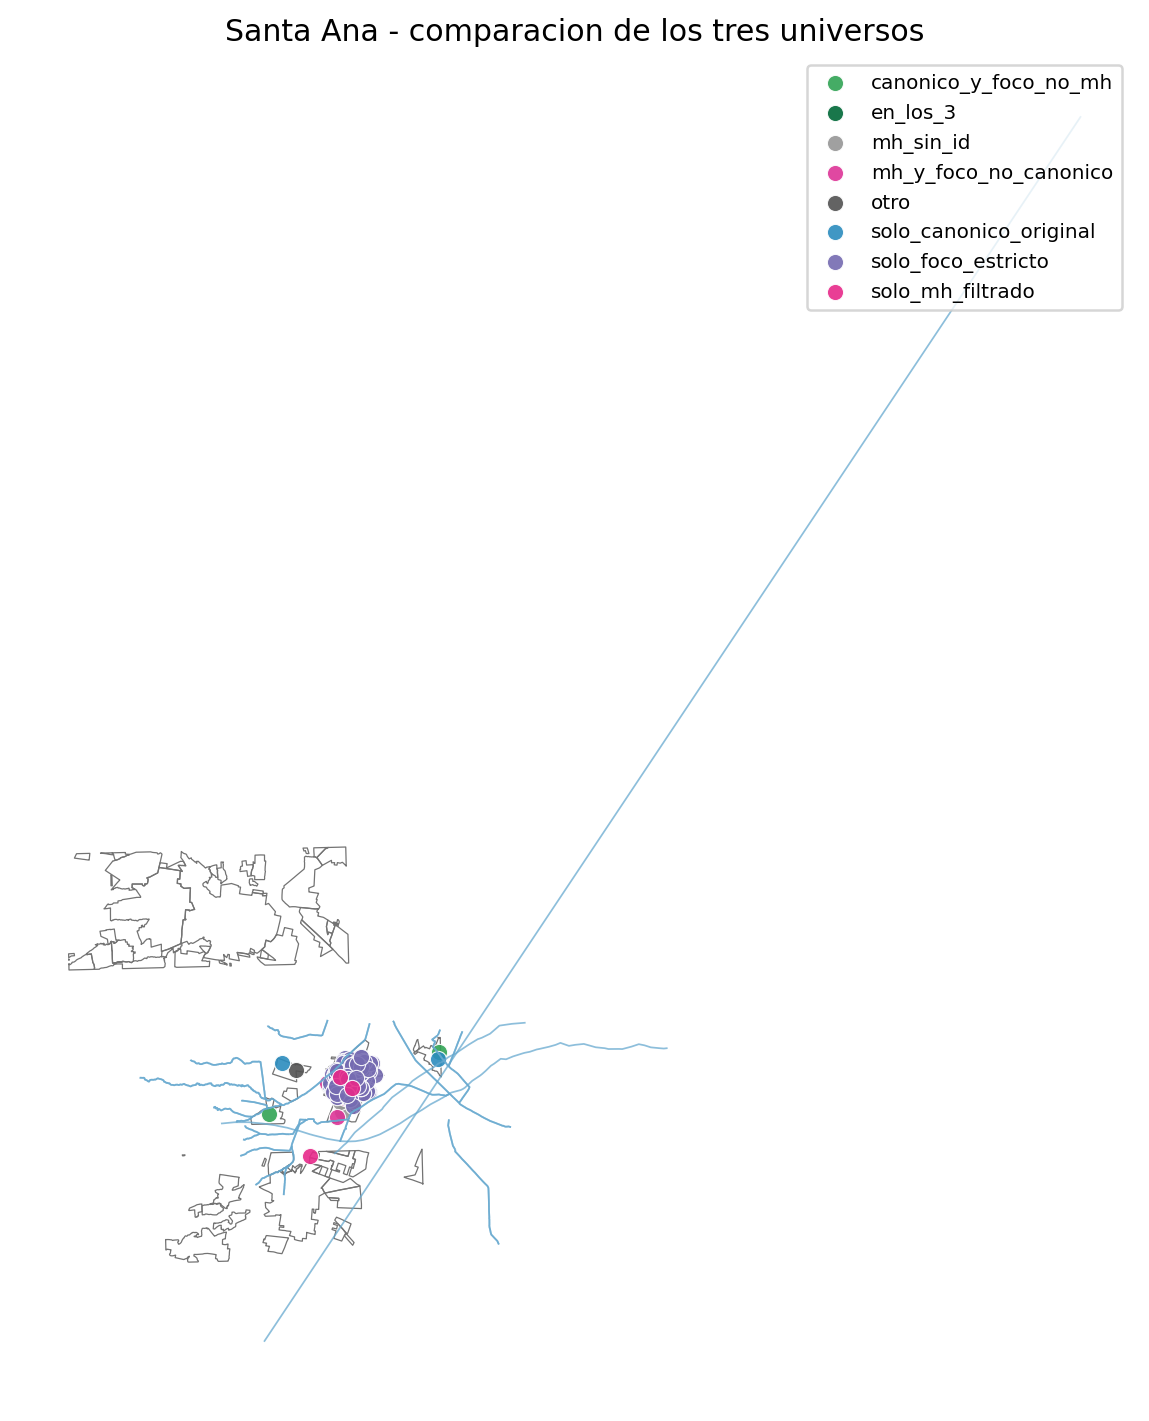
\includegraphics[width=0.95\linewidth]{../../outputs/santa_ana_xalmimilulco/mapas/mapa_comparacion_3_universos.png}

\caption{Comparación de los tres universos vigentes.}

\end{figure}

\begin{figure}[h!]\centering

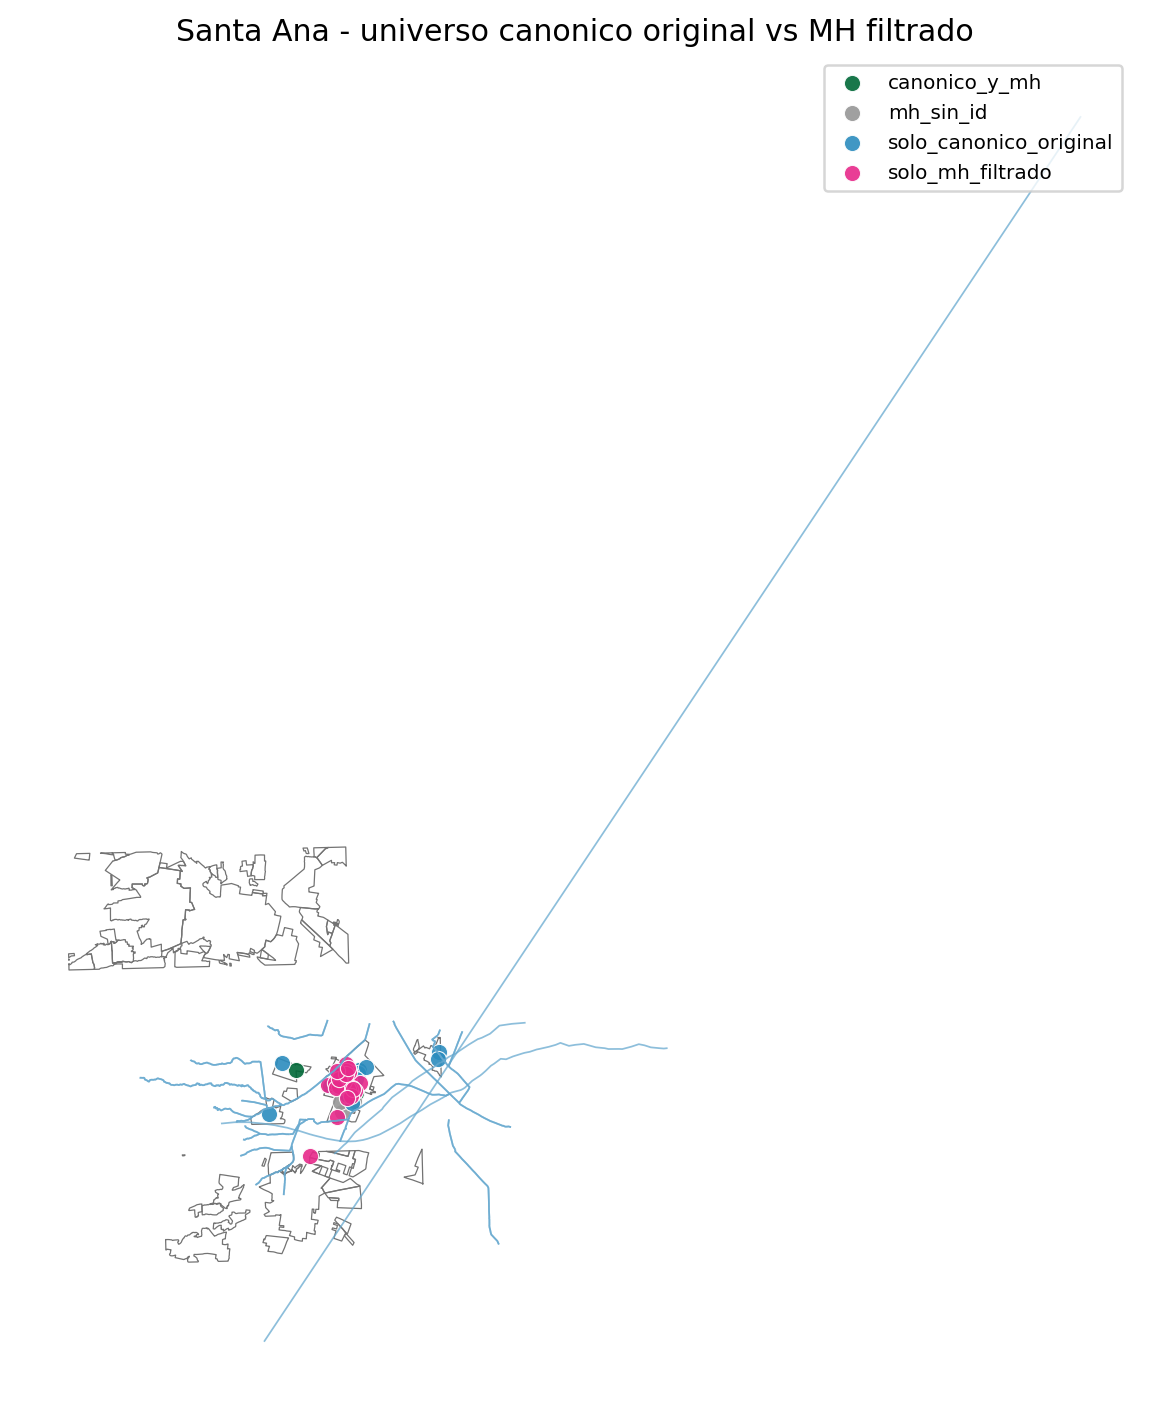
\includegraphics[width=0.95\linewidth]{../../outputs/santa_ana_xalmimilulco/mapas/mapa_canonico_original_vs_mh_filtrado.png}

\caption{Universo canónico original frente a MH filtrado.}

\end{figure}

\end{document}